\documentclass{beamer}

\usetheme{CambridgeUS}
\usefonttheme{professionalfonts}

\usepackage{graphicx}
\usepackage[miktex]{gnuplottex}
\ShellEscapetrue
\usepackage{epstopdf}
\usepackage{minted}

\usemintedstyle{manni}
\definecolor{mintedBg}{rgb}{0.98,0.98,0.70}

\begin{document}
\title{QuantLib Erlk\"onige}  
\author{Peter Caspers}
\institute{IKB}
\date{December 4th 2014} 

\frame{\titlepage} 

\begin{frame}[fragile]
\frametitle{Erlk\"onig}
\resizebox{\textwidth}{!}{
\begin{minipage}{3.5\textwidth}
\begin{figure}
	\centering
		\includegraphics{../../../Pictures/erlkoenige/Erlkoenig-VW-Golf-VII-Variant-729x486-657b2da7653d9840.jpg}
\end{figure}
\end{minipage}}
\end{frame}

\frame{\frametitle{Table of contents}\tiny\tableofcontents[hideallsubsections]} 

\section{No Arbitrage SABR}

\frame{\frametitle{No Arbitrage SABR - the model}
Paul Doust, No-arbitrage SABR, Journal of Computational Finance, Volume 15 / Number 3, Spring 2012. Main Features:
\begin{enumerate}
\item approximates the density (with a positive function), thereby producing an arbitrage free smile over strike range $[0,\infty)$
\item assumes arbsorbing barrier at $F=0$ and reproduces precomputed arbsorption probabilities generated by a MC simulation (published by Paul Doust as well)
\item call prices are computed by numerical integration, implied volatilities are computed by inverting the Black formula
\end{enumerate}
}

% %just to generate figure that is included below
% \begin{frame}[fragile]
% \begin{figure}
% 	 \begin{gnuplot}
% 	 	set terminal epslatex color
% 	 	set xrange [0:0.15]
% 	 	set yrange [-40:40]
% 	 	set xlabel "strike"
% 	 	set ylabel "density"
%         set grid
% 	 	plot 'out.txt' u 1:5 w l title 'Hagan (2002)', '' u 1:9 w l title 'Doust'
% 	 \end{gnuplot}
% \end{figure}
% \end{frame}


\frame{\frametitle{No Arbitrage SABR Example}
\resizebox{\textwidth}{!}{
\begin{minipage}{1.5\textwidth}
\begin{figure}
% GNUPLOT: LaTeX picture with Postscript
\begingroup
  \makeatletter
  \providecommand\color[2][]{%
    \GenericError{(gnuplot) \space\space\space\@spaces}{%
      Package color not loaded in conjunction with
      terminal option `colourtext'%
    }{See the gnuplot documentation for explanation.%
    }{Either use 'blacktext' in gnuplot or load the package
      color.sty in LaTeX.}%
    \renewcommand\color[2][]{}%
  }%
  \providecommand\includegraphics[2][]{%
    \GenericError{(gnuplot) \space\space\space\@spaces}{%
      Package graphicx or graphics not loaded%
    }{See the gnuplot documentation for explanation.%
    }{The gnuplot epslatex terminal needs graphicx.sty or graphics.sty.}%
    \renewcommand\includegraphics[2][]{}%
  }%
  \providecommand\rotatebox[2]{#2}%
  \@ifundefined{ifGPcolor}{%
    \newif\ifGPcolor
    \GPcolortrue
  }{}%
  \@ifundefined{ifGPblacktext}{%
    \newif\ifGPblacktext
    \GPblacktexttrue
  }{}%
  % define a \g@addto@macro without @ in the name:
  \let\gplgaddtomacro\g@addto@macro
  % define empty templates for all commands taking text:
  \gdef\gplbacktext{}%
  \gdef\gplfronttext{}%
  \makeatother
  \ifGPblacktext
    % no textcolor at all
    \def\colorrgb#1{}%
    \def\colorgray#1{}%
  \else
    % gray or color?
    \ifGPcolor
      \def\colorrgb#1{\color[rgb]{#1}}%
      \def\colorgray#1{\color[gray]{#1}}%
      \expandafter\def\csname LTw\endcsname{\color{white}}%
      \expandafter\def\csname LTb\endcsname{\color{black}}%
      \expandafter\def\csname LTa\endcsname{\color{black}}%
      \expandafter\def\csname LT0\endcsname{\color[rgb]{1,0,0}}%
      \expandafter\def\csname LT1\endcsname{\color[rgb]{0,1,0}}%
      \expandafter\def\csname LT2\endcsname{\color[rgb]{0,0,1}}%
      \expandafter\def\csname LT3\endcsname{\color[rgb]{1,0,1}}%
      \expandafter\def\csname LT4\endcsname{\color[rgb]{0,1,1}}%
      \expandafter\def\csname LT5\endcsname{\color[rgb]{1,1,0}}%
      \expandafter\def\csname LT6\endcsname{\color[rgb]{0,0,0}}%
      \expandafter\def\csname LT7\endcsname{\color[rgb]{1,0.3,0}}%
      \expandafter\def\csname LT8\endcsname{\color[rgb]{0.5,0.5,0.5}}%
    \else
      % gray
      \def\colorrgb#1{\color{black}}%
      \def\colorgray#1{\color[gray]{#1}}%
      \expandafter\def\csname LTw\endcsname{\color{white}}%
      \expandafter\def\csname LTb\endcsname{\color{black}}%
      \expandafter\def\csname LTa\endcsname{\color{black}}%
      \expandafter\def\csname LT0\endcsname{\color{black}}%
      \expandafter\def\csname LT1\endcsname{\color{black}}%
      \expandafter\def\csname LT2\endcsname{\color{black}}%
      \expandafter\def\csname LT3\endcsname{\color{black}}%
      \expandafter\def\csname LT4\endcsname{\color{black}}%
      \expandafter\def\csname LT5\endcsname{\color{black}}%
      \expandafter\def\csname LT6\endcsname{\color{black}}%
      \expandafter\def\csname LT7\endcsname{\color{black}}%
      \expandafter\def\csname LT8\endcsname{\color{black}}%
    \fi
  \fi
  \setlength{\unitlength}{0.0500bp}%
  \begin{picture}(7200.00,5040.00)%
    \gplgaddtomacro\gplbacktext{%
      \csname LTb\endcsname%
      \put(814,704){\makebox(0,0)[r]{\strut{}-40}}%
      \csname LTb\endcsname%
      \put(814,1213){\makebox(0,0)[r]{\strut{}-30}}%
      \csname LTb\endcsname%
      \put(814,1722){\makebox(0,0)[r]{\strut{}-20}}%
      \csname LTb\endcsname%
      \put(814,2231){\makebox(0,0)[r]{\strut{}-10}}%
      \csname LTb\endcsname%
      \put(814,2740){\makebox(0,0)[r]{\strut{} 0}}%
      \csname LTb\endcsname%
      \put(814,3248){\makebox(0,0)[r]{\strut{} 10}}%
      \csname LTb\endcsname%
      \put(814,3757){\makebox(0,0)[r]{\strut{} 20}}%
      \csname LTb\endcsname%
      \put(814,4266){\makebox(0,0)[r]{\strut{} 30}}%
      \csname LTb\endcsname%
      \put(814,4775){\makebox(0,0)[r]{\strut{} 40}}%
      \csname LTb\endcsname%
      \put(946,484){\makebox(0,0){\strut{} 0}}%
      \csname LTb\endcsname%
      \put(1727,484){\makebox(0,0){\strut{} 0.02}}%
      \csname LTb\endcsname%
      \put(2508,484){\makebox(0,0){\strut{} 0.04}}%
      \csname LTb\endcsname%
      \put(3289,484){\makebox(0,0){\strut{} 0.06}}%
      \csname LTb\endcsname%
      \put(4070,484){\makebox(0,0){\strut{} 0.08}}%
      \csname LTb\endcsname%
      \put(4851,484){\makebox(0,0){\strut{} 0.1}}%
      \csname LTb\endcsname%
      \put(5632,484){\makebox(0,0){\strut{} 0.12}}%
      \csname LTb\endcsname%
      \put(6413,484){\makebox(0,0){\strut{} 0.14}}%
      \put(176,2739){\rotatebox{-270}{\makebox(0,0){\strut{}density}}}%
      \put(3874,154){\makebox(0,0){\strut{}strike}}%
    }%
    \gplgaddtomacro\gplfronttext{%
      \csname LTb\endcsname%
      \put(5816,4602){\makebox(0,0)[r]{\strut{}Hagan (2002)}}%
      \csname LTb\endcsname%
      \put(5816,4382){\makebox(0,0)[r]{\strut{}Doust}}%
    }%
    \gplbacktext
    \put(0,0){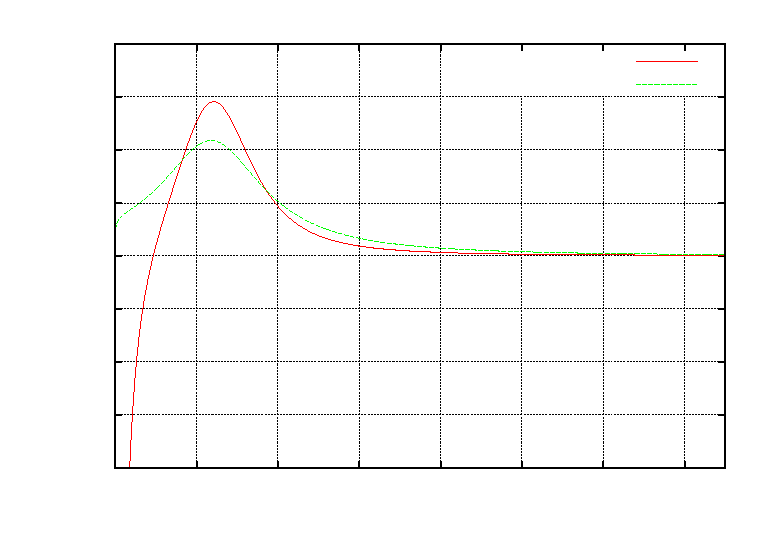
\includegraphics{qlws2014-gnuplottex-fig1}}%
    \gplfronttext
  \end{picture}%
\endgroup

\caption{SABR smile $\alpha=0.02$, $\beta=0.40$, $\nu=0.30$, $\rho=0.30$, $\tau=30.0$, $f=0.03$}
\end{figure}
\end{minipage}}
}

\begin{frame}[fragile]
\frametitle{No Arbitrage SABR classes}

\verb+ql/experimental/volatility/+

\begin{table}
\begin{tabular}{l|l}
\verb+NoArbSabrModel+ & core computation formulas \\
\verb+NoArbSabrInterpolation+ & interpolation class \\
\verb+NoArbSabrSmileSection+ & smile section by parameters \\
\verb+NoArbSabrInterpolatedSmileSection+ & interpolating smile section \\
\verb+SwaptionVolcube1a+ & volatility cube 
\end{tabular}
\end{table}
\end{frame}

\begin{frame}[fragile]
\frametitle{Design changes}
Make the SABR interpolation and volatility cube classes generic, so that both models (and possibly more like SVI, ZABR) are accepted. The old \verb+SwaptionVolCube1+ class e.g. is now retrieved by 
\vspace{2mm}
\begin{minted}[bgcolor=mintedBg]{c++}
struct SwaptionVolCubeSabrModel {
        typedef SABRInterpolation Interpolation;
        typedef SabrSmileSection SmileSection;
};

typedef SwaptionVolCube1x<SwaptionVolCubeSabrModel> 
                                      SwaptionVolCube1;

\end{minted}
\\
\vspace{2mm}
and likewise for the new ``1a''-variant of the cube using the noarb-SABR formula.
\end{frame}

\frame{\frametitle{NoArbSABR - limitations}

\begin{enumerate}
\item there are examples of parameters $(\alpha,\beta,\nu,\rho)$ for which the recalibration of the model implied forward does not work
\item the implied volatility (since inverted from call prices) is not smooth for far otm strikes in some cases (but actually rarely needed because calls, digitals and the density is directly available !)
\item in general, never underestimate the benefit of a pure closed form formula (i.e. Hagan 2002) over a computation involving numerical procedures ...
\end{enumerate}

}

\section{ZABR, SVI}

\frame{\frametitle{ZABR, SVI}
There are other models fitting in this framework like Andreasen's ZABR model
\begin{eqnarray}
dF = F^\beta \sigma dW \\
d\sigma = \nu \sigma^\gamma dV \\
dVdW = \rho dt
\end{eqnarray}
with an additional parameter $\gamma$ giving more flexibility for wing calibration to e.g. CMS quotes.
}

% %just to generate figure that is included below
% \begin{frame}[fragile]
% \begin{figure}
% 	 \begin{gnuplot}
% 	 	set terminal epslatex color
%         set xrange [*:*]
%         set yrange [*:*]
%         set xlabel "strike"
%         set ylabel "implied lognormal volatility"
%         set grid
%         plot 'out2.txt' u 1:2 w l title 'SABR', '' u 1:10 w l title 'ZABR 1.0', '' u 1:14 w l title 'ZABR 0.5', '' u 1:18 w l title 'ZABR 1.5' 
% 	 \end{gnuplot}
% \end{figure}
% \end{frame}


\frame{\frametitle{ZABR Example}
\resizebox{\textwidth}{!}{
\begin{minipage}{1.5\textwidth}
\begin{figure}
% GNUPLOT: LaTeX picture with Postscript
\begingroup
  \makeatletter
  \providecommand\color[2][]{%
    \GenericError{(gnuplot) \space\space\space\@spaces}{%
      Package color not loaded in conjunction with
      terminal option `colourtext'%
    }{See the gnuplot documentation for explanation.%
    }{Either use 'blacktext' in gnuplot or load the package
      color.sty in LaTeX.}%
    \renewcommand\color[2][]{}%
  }%
  \providecommand\includegraphics[2][]{%
    \GenericError{(gnuplot) \space\space\space\@spaces}{%
      Package graphicx or graphics not loaded%
    }{See the gnuplot documentation for explanation.%
    }{The gnuplot epslatex terminal needs graphicx.sty or graphics.sty.}%
    \renewcommand\includegraphics[2][]{}%
  }%
  \providecommand\rotatebox[2]{#2}%
  \@ifundefined{ifGPcolor}{%
    \newif\ifGPcolor
    \GPcolortrue
  }{}%
  \@ifundefined{ifGPblacktext}{%
    \newif\ifGPblacktext
    \GPblacktexttrue
  }{}%
  % define a \g@addto@macro without @ in the name:
  \let\gplgaddtomacro\g@addto@macro
  % define empty templates for all commands taking text:
  \gdef\gplbacktext{}%
  \gdef\gplfronttext{}%
  \makeatother
  \ifGPblacktext
    % no textcolor at all
    \def\colorrgb#1{}%
    \def\colorgray#1{}%
  \else
    % gray or color?
    \ifGPcolor
      \def\colorrgb#1{\color[rgb]{#1}}%
      \def\colorgray#1{\color[gray]{#1}}%
      \expandafter\def\csname LTw\endcsname{\color{white}}%
      \expandafter\def\csname LTb\endcsname{\color{black}}%
      \expandafter\def\csname LTa\endcsname{\color{black}}%
      \expandafter\def\csname LT0\endcsname{\color[rgb]{1,0,0}}%
      \expandafter\def\csname LT1\endcsname{\color[rgb]{0,1,0}}%
      \expandafter\def\csname LT2\endcsname{\color[rgb]{0,0,1}}%
      \expandafter\def\csname LT3\endcsname{\color[rgb]{1,0,1}}%
      \expandafter\def\csname LT4\endcsname{\color[rgb]{0,1,1}}%
      \expandafter\def\csname LT5\endcsname{\color[rgb]{1,1,0}}%
      \expandafter\def\csname LT6\endcsname{\color[rgb]{0,0,0}}%
      \expandafter\def\csname LT7\endcsname{\color[rgb]{1,0.3,0}}%
      \expandafter\def\csname LT8\endcsname{\color[rgb]{0.5,0.5,0.5}}%
    \else
      % gray
      \def\colorrgb#1{\color{black}}%
      \def\colorgray#1{\color[gray]{#1}}%
      \expandafter\def\csname LTw\endcsname{\color{white}}%
      \expandafter\def\csname LTb\endcsname{\color{black}}%
      \expandafter\def\csname LTa\endcsname{\color{black}}%
      \expandafter\def\csname LT0\endcsname{\color{black}}%
      \expandafter\def\csname LT1\endcsname{\color{black}}%
      \expandafter\def\csname LT2\endcsname{\color{black}}%
      \expandafter\def\csname LT3\endcsname{\color{black}}%
      \expandafter\def\csname LT4\endcsname{\color{black}}%
      \expandafter\def\csname LT5\endcsname{\color{black}}%
      \expandafter\def\csname LT6\endcsname{\color{black}}%
      \expandafter\def\csname LT7\endcsname{\color{black}}%
      \expandafter\def\csname LT8\endcsname{\color{black}}%
    \fi
  \fi
  \setlength{\unitlength}{0.0500bp}%
  \begin{picture}(7200.00,5040.00)%
    \gplgaddtomacro\gplbacktext{%
      \csname LTb\endcsname%
      \put(946,704){\makebox(0,0)[r]{\strut{} 0.1}}%
      \csname LTb\endcsname%
      \put(946,1213){\makebox(0,0)[r]{\strut{} 0.2}}%
      \csname LTb\endcsname%
      \put(946,1722){\makebox(0,0)[r]{\strut{} 0.3}}%
      \csname LTb\endcsname%
      \put(946,2231){\makebox(0,0)[r]{\strut{} 0.4}}%
      \csname LTb\endcsname%
      \put(946,2740){\makebox(0,0)[r]{\strut{} 0.5}}%
      \csname LTb\endcsname%
      \put(946,3248){\makebox(0,0)[r]{\strut{} 0.6}}%
      \csname LTb\endcsname%
      \put(946,3757){\makebox(0,0)[r]{\strut{} 0.7}}%
      \csname LTb\endcsname%
      \put(946,4266){\makebox(0,0)[r]{\strut{} 0.8}}%
      \csname LTb\endcsname%
      \put(946,4775){\makebox(0,0)[r]{\strut{} 0.9}}%
      \csname LTb\endcsname%
      \put(1078,484){\makebox(0,0){\strut{} 0}}%
      \csname LTb\endcsname%
      \put(1896,484){\makebox(0,0){\strut{} 0.1}}%
      \csname LTb\endcsname%
      \put(2714,484){\makebox(0,0){\strut{} 0.2}}%
      \csname LTb\endcsname%
      \put(3532,484){\makebox(0,0){\strut{} 0.3}}%
      \csname LTb\endcsname%
      \put(4349,484){\makebox(0,0){\strut{} 0.4}}%
      \csname LTb\endcsname%
      \put(5167,484){\makebox(0,0){\strut{} 0.5}}%
      \csname LTb\endcsname%
      \put(5985,484){\makebox(0,0){\strut{} 0.6}}%
      \csname LTb\endcsname%
      \put(6803,484){\makebox(0,0){\strut{} 0.7}}%
      \put(176,2739){\rotatebox{-270}{\makebox(0,0){\strut{}implied lognormal volatility}}}%
      \put(3940,154){\makebox(0,0){\strut{}strike}}%
    }%
    \gplgaddtomacro\gplfronttext{%
      \csname LTb\endcsname%
      \put(5816,4602){\makebox(0,0)[r]{\strut{}SABR}}%
      \csname LTb\endcsname%
      \put(5816,4382){\makebox(0,0)[r]{\strut{}ZABR 1.0}}%
      \csname LTb\endcsname%
      \put(5816,4162){\makebox(0,0)[r]{\strut{}ZABR 0.5}}%
      \csname LTb\endcsname%
      \put(5816,3942){\makebox(0,0)[r]{\strut{}ZABR 1.5}}%
    }%
    \gplbacktext
    \put(0,0){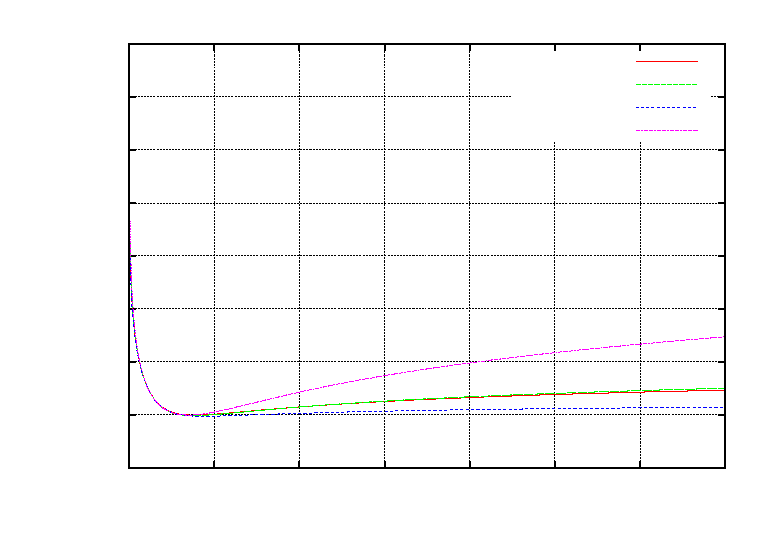
\includegraphics{qlws2014-gnuplottex-fig2}}%
    \gplfronttext
  \end{picture}%
\endgroup

\caption{SABR (Hagan 2002 expansion) $\alpha=0.03$, $\beta=0.70$, $\nu=0.20$, $\rho=-0.30$, $\tau=5.0$, $f=0.03$ vs. ZABR (short maturity expansion) for different $\gamma=0.5,1.0,1.5$ controlling the smile wings.}
\end{figure}
\end{minipage}}
}

\frame{\frametitle{ZABR - more features and limitations}

\begin{enumerate}
\item two short maturity exapnsions (normal and lognormal implied volatility)
\item an ``equivalent'' Dupire - style FD approximation, which is fast and arbitrage free in particular
\item a full finite solution, for benchmarking and testing (slow of course)
\item but ... approximations are not very good for long option expiries
\item advantages for CMS pricing yet to be proved in a productive setting 
\end{enumerate}

}

\frame{\frametitle{SVI}
SVI is another popular smile model, with the total variance given by
\begin{equation}
v^2t = a + b (\rho (k-m) + \sqrt{(k-m)^2+\sigma^2})
\end{equation}
with log moneyness $k = \log K / F$, $K$ = strike, $F$ = forward.
}

% %just to generate figure that is included below
% \begin{frame}[fragile]
% \begin{figure}
% 	 \begin{gnuplot}
% 	 	set terminal epslatex color
%         set xrange [*:*]
%         set yrange [*:*]
%         set xlabel "strike"
%         set ylabel "implied lognormal volatility"
%         set grid
%         plot 'out3.txt' u 1:2 w p title 'Input', 'out4.txt' u 1:2 w l title 'SVI'
% 	 \end{gnuplot}
% \end{figure}
% \end{frame}

\frame{\frametitle{SVI Example}
\resizebox{\textwidth}{!}{
\begin{minipage}{1.5\textwidth}
\begin{figure}
% GNUPLOT: LaTeX picture with Postscript
\begingroup
  \makeatletter
  \providecommand\color[2][]{%
    \GenericError{(gnuplot) \space\space\space\@spaces}{%
      Package color not loaded in conjunction with
      terminal option `colourtext'%
    }{See the gnuplot documentation for explanation.%
    }{Either use 'blacktext' in gnuplot or load the package
      color.sty in LaTeX.}%
    \renewcommand\color[2][]{}%
  }%
  \providecommand\includegraphics[2][]{%
    \GenericError{(gnuplot) \space\space\space\@spaces}{%
      Package graphicx or graphics not loaded%
    }{See the gnuplot documentation for explanation.%
    }{The gnuplot epslatex terminal needs graphicx.sty or graphics.sty.}%
    \renewcommand\includegraphics[2][]{}%
  }%
  \providecommand\rotatebox[2]{#2}%
  \@ifundefined{ifGPcolor}{%
    \newif\ifGPcolor
    \GPcolortrue
  }{}%
  \@ifundefined{ifGPblacktext}{%
    \newif\ifGPblacktext
    \GPblacktexttrue
  }{}%
  % define a \g@addto@macro without @ in the name:
  \let\gplgaddtomacro\g@addto@macro
  % define empty templates for all commands taking text:
  \gdef\gplbacktext{}%
  \gdef\gplfronttext{}%
  \makeatother
  \ifGPblacktext
    % no textcolor at all
    \def\colorrgb#1{}%
    \def\colorgray#1{}%
  \else
    % gray or color?
    \ifGPcolor
      \def\colorrgb#1{\color[rgb]{#1}}%
      \def\colorgray#1{\color[gray]{#1}}%
      \expandafter\def\csname LTw\endcsname{\color{white}}%
      \expandafter\def\csname LTb\endcsname{\color{black}}%
      \expandafter\def\csname LTa\endcsname{\color{black}}%
      \expandafter\def\csname LT0\endcsname{\color[rgb]{1,0,0}}%
      \expandafter\def\csname LT1\endcsname{\color[rgb]{0,1,0}}%
      \expandafter\def\csname LT2\endcsname{\color[rgb]{0,0,1}}%
      \expandafter\def\csname LT3\endcsname{\color[rgb]{1,0,1}}%
      \expandafter\def\csname LT4\endcsname{\color[rgb]{0,1,1}}%
      \expandafter\def\csname LT5\endcsname{\color[rgb]{1,1,0}}%
      \expandafter\def\csname LT6\endcsname{\color[rgb]{0,0,0}}%
      \expandafter\def\csname LT7\endcsname{\color[rgb]{1,0.3,0}}%
      \expandafter\def\csname LT8\endcsname{\color[rgb]{0.5,0.5,0.5}}%
    \else
      % gray
      \def\colorrgb#1{\color{black}}%
      \def\colorgray#1{\color[gray]{#1}}%
      \expandafter\def\csname LTw\endcsname{\color{white}}%
      \expandafter\def\csname LTb\endcsname{\color{black}}%
      \expandafter\def\csname LTa\endcsname{\color{black}}%
      \expandafter\def\csname LT0\endcsname{\color{black}}%
      \expandafter\def\csname LT1\endcsname{\color{black}}%
      \expandafter\def\csname LT2\endcsname{\color{black}}%
      \expandafter\def\csname LT3\endcsname{\color{black}}%
      \expandafter\def\csname LT4\endcsname{\color{black}}%
      \expandafter\def\csname LT5\endcsname{\color{black}}%
      \expandafter\def\csname LT6\endcsname{\color{black}}%
      \expandafter\def\csname LT7\endcsname{\color{black}}%
      \expandafter\def\csname LT8\endcsname{\color{black}}%
    \fi
  \fi
  \setlength{\unitlength}{0.0500bp}%
  \begin{picture}(7200.00,5040.00)%
    \gplgaddtomacro\gplbacktext{%
      \csname LTb\endcsname%
      \put(1078,704){\makebox(0,0)[r]{\strut{} 0.2}}%
      \csname LTb\endcsname%
      \put(1078,1156){\makebox(0,0)[r]{\strut{} 0.25}}%
      \csname LTb\endcsname%
      \put(1078,1609){\makebox(0,0)[r]{\strut{} 0.3}}%
      \csname LTb\endcsname%
      \put(1078,2061){\makebox(0,0)[r]{\strut{} 0.35}}%
      \csname LTb\endcsname%
      \put(1078,2513){\makebox(0,0)[r]{\strut{} 0.4}}%
      \csname LTb\endcsname%
      \put(1078,2966){\makebox(0,0)[r]{\strut{} 0.45}}%
      \csname LTb\endcsname%
      \put(1078,3418){\makebox(0,0)[r]{\strut{} 0.5}}%
      \csname LTb\endcsname%
      \put(1078,3870){\makebox(0,0)[r]{\strut{} 0.55}}%
      \csname LTb\endcsname%
      \put(1078,4323){\makebox(0,0)[r]{\strut{} 0.6}}%
      \csname LTb\endcsname%
      \put(1078,4775){\makebox(0,0)[r]{\strut{} 0.65}}%
      \csname LTb\endcsname%
      \put(1210,484){\makebox(0,0){\strut{} 0}}%
      \csname LTb\endcsname%
      \put(1769,484){\makebox(0,0){\strut{} 0.01}}%
      \csname LTb\endcsname%
      \put(2329,484){\makebox(0,0){\strut{} 0.02}}%
      \csname LTb\endcsname%
      \put(2888,484){\makebox(0,0){\strut{} 0.03}}%
      \csname LTb\endcsname%
      \put(3447,484){\makebox(0,0){\strut{} 0.04}}%
      \csname LTb\endcsname%
      \put(4007,484){\makebox(0,0){\strut{} 0.05}}%
      \csname LTb\endcsname%
      \put(4566,484){\makebox(0,0){\strut{} 0.06}}%
      \csname LTb\endcsname%
      \put(5125,484){\makebox(0,0){\strut{} 0.07}}%
      \csname LTb\endcsname%
      \put(5684,484){\makebox(0,0){\strut{} 0.08}}%
      \csname LTb\endcsname%
      \put(6244,484){\makebox(0,0){\strut{} 0.09}}%
      \csname LTb\endcsname%
      \put(6803,484){\makebox(0,0){\strut{} 0.1}}%
      \put(176,2739){\rotatebox{-270}{\makebox(0,0){\strut{}implied lognormal volatility}}}%
      \put(4006,154){\makebox(0,0){\strut{}strike}}%
    }%
    \gplgaddtomacro\gplfronttext{%
      \csname LTb\endcsname%
      \put(5816,4602){\makebox(0,0)[r]{\strut{}Input}}%
      \csname LTb\endcsname%
      \put(5816,4382){\makebox(0,0)[r]{\strut{}SVI}}%
    }%
    \gplbacktext
    \put(0,0){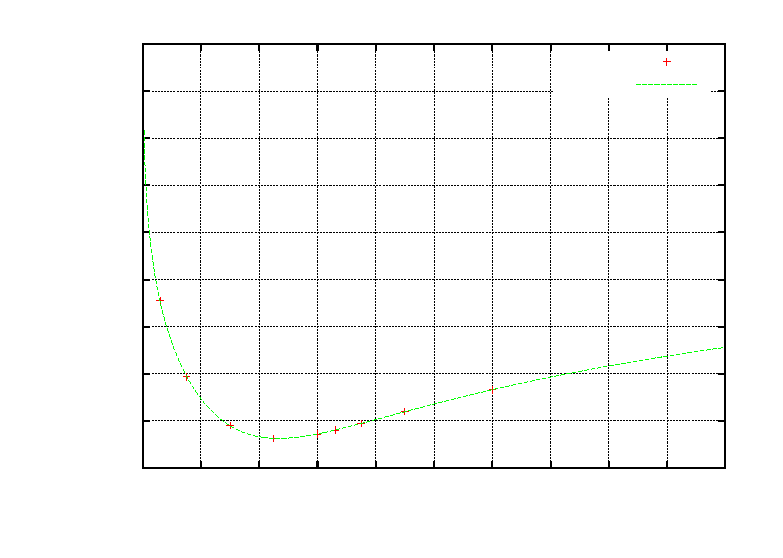
\includegraphics{qlws2014-gnuplottex-fig3}}%
    \gplfronttext
  \end{picture}%
\endgroup

\caption{SVI fit to sample input data generated by SABR ($\alpha=0.08$, $\beta=0.90$, $\nu=0.30$, $\rho=0.30$, $\tau=10.0$, $f=0.03$)}
\end{figure}
\end{minipage}}
}

\begin{frame}[fragile]
\frametitle{Implementation of SVI 1/2}
We can use the generic framework, so e.g. the implementation of the SVI interpolation class is merely specifying the SVI specific things ...
\vspace{2mm}
\begin{minted}[bgcolor=mintedBg, fontsize=\tiny]{c++}
typedef SviSmileSection SviWrapper;
struct SviSpecs {
    Size dimension() { return 5; }
    void defaultValues(std::vector<Real> &params, std::vector<bool> &paramIsFixed,
                       const Real &forward, const Real expiryTime) { /* ... */ }
    void guess(Array &values, const std::vector<bool> &paramIsFixed,
               const Real &forward, const Real expiryTime,
               const std::vector<Real> &r) { /* ... */ }
    Array inverse(const Array &y, const std::vector<bool> &,
                  const std::vector<Real> &, const Real) { /* ... */  }
    Array direct(const Array &x, const std::vector<bool> &paramIsFixed,
                 const std::vector<Real> &params, const Real forward) { /* ... */ }
    typedef SviWrapper type;
    boost::shared_ptr<type> instance(const Time t, const Real &forward,
                                     const std::vector<Real> &params) { /* ... */ }
};
\end{minted}
\end{frame}

\begin{frame}[fragile]
\frametitle{Implementation of SVI (2/2)}
... and use this in the generic implemenation:
\vspace{2mm}
\begin{minted}[bgcolor=mintedBg, fontsize=\tiny]{c++}
class SviInterpolation : public Interpolation {
  public:
    template <class I1, class I2>
    SviInterpolation(const I1 &xBegin, ... ) {
        impl_ = boost::shared_ptr<Interpolation::Impl>(
            new detail::XABRInterpolationImpl<I1, I2, detail::SviSpecs>(
                xBegin, xEnd, yBegin, t, forward,
                boost::assign::list_of(a)(b)(sigma)(rho)(m),
                boost::assign::list_of(aIsFixed)(bIsFixed)(sigmaIsFixed)(
                    rhoIsFixed)(mIsFixed),
                vegaWeighted, endCriteria, optMethod, errorAccept, useMaxError,
                maxGuesses));
        coeffs_ = boost::dynamic_pointer_cast<
            detail::XABRCoeffHolder<detail::SviSpecs> >(impl_);
    }
\end{minted}
\\
\vspace{2mm}
Note that \verb+XABR...+ is already to narrow as the label for the generic class. Better than the other way round ...
\end{frame}

\frame{\frametitle{SVI - limitations}

\begin{enumerate}
\item uses the ``raw'' parametrization, which does not allow for easy parameter interpretation
\item calibration is naive, i.e. does not avoid local minima / parameter identifcation problem cases
\end{enumerate}

}

\frame{\frametitle{Other smile models, general thoughts}
There are other models, that are not fitted, but interpolate given points by construction such that
the resulting smile is arbitrage free, e.g.

\begin{enumerate}
\item KahaleSmileSection which is already used implicity by the Markov functional model
\item BDK which fixes arbitrageable wings and introduce new parameters for wing calibration
\end{enumerate}

Goal: Integrate them as well in a uniform infrastructure providing

\begin{enumerate}
\item an interpolation class
\item a smile section which takes either parameters, market data or a source smile section to be smoothed / made arb-free
\item a swaption volatility cube with the possibility to calibrate to the cms market and a caplet volatility surface
\end{enumerate}
}

\section{Linear TSR CMS Coupon Pricer}

\frame{\frametitle{TSR CMS Coupon Pricers}
A terminal swap rate (TSR) model is given by a mapping $\alpha$
\begin{equation}
\alpha( S(t) ) = \frac{P(t,t_P)}{A(t)}
\end{equation}
where $t_p$ is the coupon payment date and $A(t)$ the annuity of the underlying swap rate $S$. Then (integration by parts) the
npv of a general CMS coupon $A(0) E^A( P(t,t_p) / A(t) g(S(t)) )$ is given by 
\begin{equation}
A(0)S(0)\alpha(S(0))+\int_{-\infty}^{S(0)} w(k)R(k)dk+\int_{S(0)}^\infty w(k)P(k)dk
\end{equation}
with $t$ begin the fixing date of the coupon, $R$ and $P$ prices of market receiver and payer swaptions and weights $w(s)=\{\alpha(s)g(s)\}''.$
}

\frame{\frametitle{Hagan non parallel shifts model}
In Hagan's classic paper, the model A.4 ``non parallel shifts'' corresponds to the following choice of $\alpha$
\begin{equation}
\alpha( S ) = \frac{S e^{-|h(t_p)-h(t)|x}}{1-\frac{P(0,t_n)}{P(0,t)}e^{-|h(t_n)-h(t)|x}}
\end{equation}
with $t_n$ being the last payment date of the underyling swap and $h(s)-h(t)=\frac{1-e^{-\kappa(s-t)}}{\kappa}$ with a mean reversion parameter $\kappa$ and $x$ implicitly given by
\begin{equation}
S(t) \sum \tau_jP(0,t_j)e^{-|h(t_j)-h(t)|x}+P(0,t_n)e^{-|h(t_n)-h(t)|x} = P(0,t)
\end{equation}
with $\tau_j, t_j$ being the yearfractions and payment dates of the fixed leg of the underlying swap.
}

\frame{\frametitle{Linear TSR model}
The linear terminal swap rate model is defined by

\begin{equation}
\alpha( S ) = a s + b
\end{equation}

$b$ is determined by the no arbitrage condition 

\begin{equation}
P(0,t_p)/A(0) = E^A(P(t,t_p)/A(t)) = a S(0) + b
\end{equation}

$a$ can be specified indirectly via a reversion $\kappa$ by setting

\begin{equation}
a = \frac{\partial}{\partial S(t)}\frac{P(t,t_p)}{A(t)}
\end{equation}

and evaluating the r.h.s. within a one factor gaussian model.
}

% %just to generate figure that is included below
% \begin{frame}[fragile]
% \begin{figure}
% 	 \begin{gnuplot}
%        set terminal epslatex color
%        set xrange [*:*]
%        set yrange [*:*]
%        set xlabel "strike"
%        set ylabel "put call parity violation"
%        set grid
%        set logscale y
%        set format y "%1.0e"
%        set key below
%        plot 'out5.txt' u 1:(abs($4)) w l title 'Hagan (Numeric, NonParallelShifts)', 'out6.txt' u 1:(abs($4)) w l title 'Linear TSR'
% 	 \end{gnuplot}
% \end{figure}
% \end{frame}


\frame{\frametitle{Put Call Parity Example}
\resizebox{\textwidth}{!}{
\begin{minipage}{1.5\textwidth}
\begin{figure}
% GNUPLOT: LaTeX picture with Postscript
\begingroup
  \makeatletter
  \providecommand\color[2][]{%
    \GenericError{(gnuplot) \space\space\space\@spaces}{%
      Package color not loaded in conjunction with
      terminal option `colourtext'%
    }{See the gnuplot documentation for explanation.%
    }{Either use 'blacktext' in gnuplot or load the package
      color.sty in LaTeX.}%
    \renewcommand\color[2][]{}%
  }%
  \providecommand\includegraphics[2][]{%
    \GenericError{(gnuplot) \space\space\space\@spaces}{%
      Package graphicx or graphics not loaded%
    }{See the gnuplot documentation for explanation.%
    }{The gnuplot epslatex terminal needs graphicx.sty or graphics.sty.}%
    \renewcommand\includegraphics[2][]{}%
  }%
  \providecommand\rotatebox[2]{#2}%
  \@ifundefined{ifGPcolor}{%
    \newif\ifGPcolor
    \GPcolortrue
  }{}%
  \@ifundefined{ifGPblacktext}{%
    \newif\ifGPblacktext
    \GPblacktexttrue
  }{}%
  % define a \g@addto@macro without @ in the name:
  \let\gplgaddtomacro\g@addto@macro
  % define empty templates for all commands taking text:
  \gdef\gplbacktext{}%
  \gdef\gplfronttext{}%
  \makeatother
  \ifGPblacktext
    % no textcolor at all
    \def\colorrgb#1{}%
    \def\colorgray#1{}%
  \else
    % gray or color?
    \ifGPcolor
      \def\colorrgb#1{\color[rgb]{#1}}%
      \def\colorgray#1{\color[gray]{#1}}%
      \expandafter\def\csname LTw\endcsname{\color{white}}%
      \expandafter\def\csname LTb\endcsname{\color{black}}%
      \expandafter\def\csname LTa\endcsname{\color{black}}%
      \expandafter\def\csname LT0\endcsname{\color[rgb]{1,0,0}}%
      \expandafter\def\csname LT1\endcsname{\color[rgb]{0,1,0}}%
      \expandafter\def\csname LT2\endcsname{\color[rgb]{0,0,1}}%
      \expandafter\def\csname LT3\endcsname{\color[rgb]{1,0,1}}%
      \expandafter\def\csname LT4\endcsname{\color[rgb]{0,1,1}}%
      \expandafter\def\csname LT5\endcsname{\color[rgb]{1,1,0}}%
      \expandafter\def\csname LT6\endcsname{\color[rgb]{0,0,0}}%
      \expandafter\def\csname LT7\endcsname{\color[rgb]{1,0.3,0}}%
      \expandafter\def\csname LT8\endcsname{\color[rgb]{0.5,0.5,0.5}}%
    \else
      % gray
      \def\colorrgb#1{\color{black}}%
      \def\colorgray#1{\color[gray]{#1}}%
      \expandafter\def\csname LTw\endcsname{\color{white}}%
      \expandafter\def\csname LTb\endcsname{\color{black}}%
      \expandafter\def\csname LTa\endcsname{\color{black}}%
      \expandafter\def\csname LT0\endcsname{\color{black}}%
      \expandafter\def\csname LT1\endcsname{\color{black}}%
      \expandafter\def\csname LT2\endcsname{\color{black}}%
      \expandafter\def\csname LT3\endcsname{\color{black}}%
      \expandafter\def\csname LT4\endcsname{\color{black}}%
      \expandafter\def\csname LT5\endcsname{\color{black}}%
      \expandafter\def\csname LT6\endcsname{\color{black}}%
      \expandafter\def\csname LT7\endcsname{\color{black}}%
      \expandafter\def\csname LT8\endcsname{\color{black}}%
    \fi
  \fi
  \setlength{\unitlength}{0.0500bp}%
  \begin{picture}(7200.00,5040.00)%
    \gplgaddtomacro\gplbacktext{%
      \csname LTb\endcsname%
      \put(1078,1364){\makebox(0,0)[r]{\strut{}1e-18}}%
      \csname LTb\endcsname%
      \put(1078,1851){\makebox(0,0)[r]{\strut{}1e-16}}%
      \csname LTb\endcsname%
      \put(1078,2339){\makebox(0,0)[r]{\strut{}1e-14}}%
      \csname LTb\endcsname%
      \put(1078,2826){\makebox(0,0)[r]{\strut{}1e-12}}%
      \csname LTb\endcsname%
      \put(1078,3313){\makebox(0,0)[r]{\strut{}1e-10}}%
      \csname LTb\endcsname%
      \put(1078,3800){\makebox(0,0)[r]{\strut{}1e-08}}%
      \csname LTb\endcsname%
      \put(1078,4288){\makebox(0,0)[r]{\strut{}1e-06}}%
      \csname LTb\endcsname%
      \put(1078,4775){\makebox(0,0)[r]{\strut{}1e-04}}%
      \csname LTb\endcsname%
      \put(1210,1144){\makebox(0,0){\strut{} 0}}%
      \csname LTb\endcsname%
      \put(1769,1144){\makebox(0,0){\strut{} 0.01}}%
      \csname LTb\endcsname%
      \put(2329,1144){\makebox(0,0){\strut{} 0.02}}%
      \csname LTb\endcsname%
      \put(2888,1144){\makebox(0,0){\strut{} 0.03}}%
      \csname LTb\endcsname%
      \put(3447,1144){\makebox(0,0){\strut{} 0.04}}%
      \csname LTb\endcsname%
      \put(4007,1144){\makebox(0,0){\strut{} 0.05}}%
      \csname LTb\endcsname%
      \put(4566,1144){\makebox(0,0){\strut{} 0.06}}%
      \csname LTb\endcsname%
      \put(5125,1144){\makebox(0,0){\strut{} 0.07}}%
      \csname LTb\endcsname%
      \put(5684,1144){\makebox(0,0){\strut{} 0.08}}%
      \csname LTb\endcsname%
      \put(6244,1144){\makebox(0,0){\strut{} 0.09}}%
      \csname LTb\endcsname%
      \put(6803,1144){\makebox(0,0){\strut{} 0.1}}%
      \put(176,3069){\rotatebox{-270}{\makebox(0,0){\strut{}put call parity violation}}}%
      \put(4006,814){\makebox(0,0){\strut{}strike}}%
    }%
    \gplgaddtomacro\gplfronttext{%
      \csname LTb\endcsname%
      \put(5823,393){\makebox(0,0)[r]{\strut{}Hagan (Numeric, NonParallelShifts)}}%
      \csname LTb\endcsname%
      \put(5823,173){\makebox(0,0)[r]{\strut{}Linear TSR}}%
    }%
    \gplbacktext
    \put(0,0){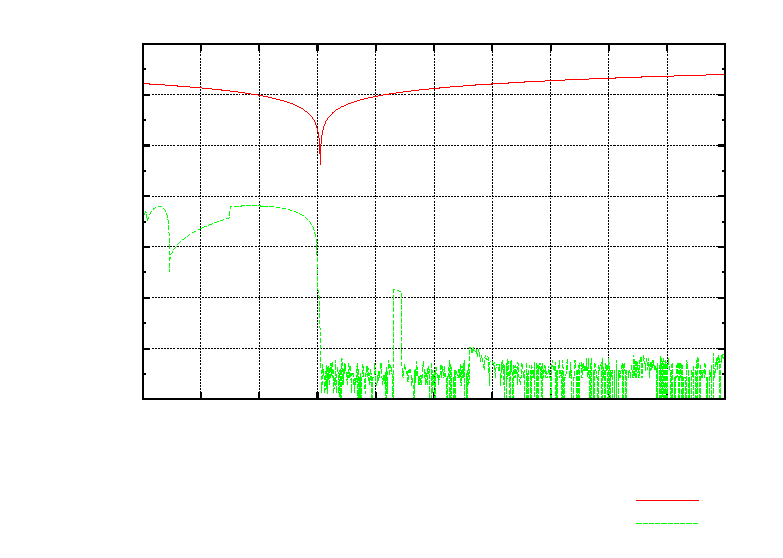
\includegraphics{qlws2014-gnuplottex-fig4}}%
    \gplfronttext
  \end{picture}%
\endgroup

\caption{Parity error for a CMS10y coupon with in arrears fixing in 10y from today, Forward is $0.03$, Volatility is given by a SABR surface with  $\alpha=0.10$, $\beta=0.80$, $\nu=0.40$, $\rho=-0.30$, reversion is zero, Integration Accuracy for the Linear TSR pricer is $10^{-10}$}
\end{figure}
\end{minipage}}
}


\begin{frame}[fragile]
\frametitle{Performance}
Computation time for pricing of 4000 optionlets (parameters as before) on Intel(R) Core(TM) i7-2760QM CPU @ 2.40GHz, single threaded.

\begin{table}
\begin{tabular}{l|r}
\verb NumericHaganPricer (Standard) & 1840ms \\
\verb NumericHaganPricer (NonParallelShifts) & 5882ms \\
\verb AnalyticHaganPricer (Standard) & 770ms \\
\verb AnalyticHaganPricer (NonParallelShifts) & 741ms \\
\verb LinearTsrPricer & 505ms
\end{tabular}
\end{table}
\end{frame}

\begin{frame}[fragile]
\frametitle{Fast Erlk\"onig}
\resizebox{\textwidth}{!}{
\begin{minipage}{5.0\textwidth}
\begin{figure}
	\centering
		\includegraphics{../../../Pictures/erlkoenige/THORIUM_fueled_car.jpg}
\end{figure}
\end{minipage}}
\end{frame}

\section{CMS Spread Coupons}

\frame{\frametitle{CMS Spread Coupons}
Still missing: a coupon class which models cms spread coupons
\begin{equation}
\tau (\textnormal{CMS10y} - \textnormal{CMS2y})
\end{equation}
possibly capped and / or floored.
}

\begin{frame}[fragile]
\frametitle{Approach 1: Formula index}
Introduce an artificial index derived from \verb+InterestRateIndex+
\vspace{2mm}
\begin{minted}[fontsize=\footnotesize, bgcolor=mintedBg]{c++}
SwapSpreadIndex(const std::string& familyName,
                const boost::shared_ptr<SwapIndex>& swapIndex1,
                const boost::shared_ptr<SwapIndex>& swapIndex2,
                const Real gearing1 = 1.0,
                const Real gearing2 = -1.0);
\end{minted}
\\
\vspace{2mm}
and build everything else on top of it as with the other coupons based
on ibor or cms indexes.
\end{frame}

\begin{frame}[fragile]
\frametitle{Approach 1: Repairing the class hiearchy}
Since the formula index does not have own fixings, we would have to
adjust the index base class by adding
\vspace{2mm}
\begin{minted}[fontsize=\footnotesize, bgcolor=mintedBg]{c++}
//! check if index allows for native fixings
virtual void checkNativeFixingsAllowed() {}
\end{minted}
\\
\vspace{2mm}
and forbid native fixings in formula based indices
\vspace{2mm}
\begin{minted}[fontsize=\footnotesize, bgcolor=mintedBg]{c++}
//! check if index allows for native fixings
virtual void checkNativeFixingsAllowed() {}
void checkNativeFixingsAllowed() {
    QL_FAIL("native fixings not allowed in swap spread index, refer to "
            "underlying indices instead");
}
\end{minted}
\\
\vspace{2mm}
A nicer solution would be to make the addFixing methods virtual and throw
an exception in CMS spread index, but they are template methods.
\end{frame}

\begin{frame}[fragile]
\frametitle{Approach 2: Construct coupons with two swap indexes}
If two swap indexes are used to construct a cms spread coupon we would need
a more flexible way to construct floating legs, since
\vspace{2mm}
\begin{minted}[fontsize=\footnotesize, bgcolor=mintedBg]{c++}
 template <typename InterestRateIndexType,
           typename FloatingCouponType,
           typename CappedFlooredCouponType>
 Leg FloatingLeg(const Schedule& schedule,
                 const std::vector<Real>& nominals,
                 const boost::shared_ptr<InterestRateIndexType>& index,
                 const DayCounter& paymentDayCounter,
                 BusinessDayConvention paymentAdj,
                 const std::vector<Natural>& fixingDays,
                 const std::vector<Real>& gearings,
                 const std::vector<Spread>& spreads,
                 const std::vector<Rate>& caps,
                 const std::vector<Rate>& floors,
                 bool isInArrears, bool isZero) {
\end{minted}
\\
\vspace{2mm}
only allows for one index. 
\end{frame}

\begin{frame}[fragile]
\frametitle{Approach 2: Coupon Factories}
We could introduce a factory instead of the template parameters
\vspace{2mm}
\begin{minted}[fontsize=\footnotesize, bgcolor=mintedBg]{c++}
Leg FloatingLeg(const FloatingCouponFactory& factory,
                const Schedule& schedule,
                ...
\end{minted}
\\
\vspace{2mm}
which can generate plain, capped / floored and digital
couons for the ibor, cms, cms spread flavours.
\vspace{2mm}
\begin{minted}[fontsize=\footnotesize, bgcolor=mintedBg]{c++}
  class FloatingCouponFactory {
    virtual boost::shared_ptr<FloatingRateCoupon>
      plainCoupon(const Date &paymentDate, Real nominal,...)
    virtual boost::shared_ptr<CappedFlooredCoupon>
      cappedFlooredCoupon(const Date &paymentDate, Real nominal,...)
    virtual boost::shared_ptr<DigitalCoupon> digitalCoupon(
      const Date &paymentDate, Real nominal, const Date &startDate,...)
    virtual Natural defaultFixingDays() const = 0;
};
\end{minted}

\end{frame}

\frame{\frametitle{CMS Spread Coupons - Summary}
\begin{itemize}
\item Introducing a formula based index would not exactly fit the semantics
of the Index class. We would have to distinguish between native
indexes (with own fixings) and derived ones. On the other hand this seems to be a quite generic approach, since formula based indexes could be used whereever an InterestRateIndex is allowed
\item Using two indexes in the spread coupon class forces us to introduce a more
flexible way to construct floating legs, e.g. via factories. This keeps the design clean and the semantics of index sharp. However this is not 100\% backward compatible since FloatingLeg is in the main QuantLib namespace.
\end{itemize}
}

\section{Credit Risk Plus}

\begin{frame}[fragile]
\frametitle{Credit Risk Plus}
A single period, nominal based credit portfolio model, based on Credit Risk Plus, with some extensions allowing for correlated sectors (Integrating Correlations, Risk, July 1999).
\vspace{2mm}
\begin{minted}[fontsize=\footnotesize, bgcolor=mintedBg]{c++}
  CreditRiskPlus(const std::vector<Real> &exposure,
     const std::vector<Real> &defaultProbability,
     const std::vector<Size> &sector,
     const std::vector<Real> &relativeDefaultVariance,
     const Matrix &correlation, const Real unit);
\end{minted}
\\
\vspace{2mm}
The loss distribution is computed analytically, so very fast. The model comes with a decomposition of the unexpected loss into single obligors' marginal losses.
\end{frame}



\section{Gaussian1d Models}

\begin{frame}[fragile]
\frametitle{Gaussian1d Models}
Framework for one factor models with the following interface

\begin{minted}[bgcolor=mintedBg,fontsize=\footnotesize]{c++}
  virtual const Real numeraireImpl(const Time t, const Real y,
                     const Handle<YieldTermStructure> &yts) const = 0;
  virtual const Real zerobondImpl(const Time T, const Time t, 
                     const Real y,
                     const Handle<YieldTermStructure> &yts) const = 0;
\end{minted}

Currently two instances exist

\begin{enumerate}
\item \verb+MarkovFunctional+, a non parametric Markov functional model with piecewise volatility and constant reversion
\item \verb+Gsr+, a Hull White model with piecewise volatility and piecewise reversion
\end{enumerate}
\end{frame}


\begin{frame}[fragile]
\frametitle{Gaussian1d Models - Features}
\begin{enumerate}
\item multi-curve enabled
\item engines for standard swaptions, swaptions with non-constant nominal, rates, float-float swaptions
\item engines inherit from \verb+BasketGeneratingEngine+ that can generate calibration baskets by npv-delta-gamma matching
\item engines take an OAS allowing for exotic bond valuation
\end{enumerate}

\end{frame}





\section{Simulated Annealing}

\frame{\frametitle{Simulated Annealing}
A global optimizer based on Nelder-Mead and additional noise in the target function. 
\begin{enumerate}
\item the noise is exponentially distributed with parameter $1/T$ (``Temperature''), i.e. the expectation and the standard deviation of the noise is both $T$
\item the optimization starts with a temperature $T>0$ which decreases to zero during the optimization
\item if the start temperature is high enough and the decrease is slow enough, a global minimum is found with probability one
\end{enumerate}
}

% %just to generate figure that is included below
% \begin{frame}[fragile]
% \begin{figure}
% 	 \begin{gnuplot}
%        set terminal epslatex color
%        set xrange [-5:5]
%        set yrange [-5:5]
%        set cbrange [0:0.5]
%        set xlabel "x"
%        set ylabel "y"
%        set zlabel "z" 
%        set isosample 100,100
%        unset key
%        set view 35,24
%        splot (sin(pi*(x+0.5))*cos(pi*(y+1))+2)*(x**2+y**2)/50.0 with pm3d, (sin(pi*(x+0.5))*cos(pi*(y+1))+2)*(x**2+y**2)/50.0 with lines 
% 	 \end{gnuplot}
% \end{figure}
% \end{frame}


\frame{\frametitle{Global optimization test function}
\resizebox{\textwidth}{!}{
\begin{minipage}{1.5\textwidth}
\begin{figure}
% GNUPLOT: LaTeX picture with Postscript
\begingroup
  \makeatletter
  \providecommand\color[2][]{%
    \GenericError{(gnuplot) \space\space\space\@spaces}{%
      Package color not loaded in conjunction with
      terminal option `colourtext'%
    }{See the gnuplot documentation for explanation.%
    }{Either use 'blacktext' in gnuplot or load the package
      color.sty in LaTeX.}%
    \renewcommand\color[2][]{}%
  }%
  \providecommand\includegraphics[2][]{%
    \GenericError{(gnuplot) \space\space\space\@spaces}{%
      Package graphicx or graphics not loaded%
    }{See the gnuplot documentation for explanation.%
    }{The gnuplot epslatex terminal needs graphicx.sty or graphics.sty.}%
    \renewcommand\includegraphics[2][]{}%
  }%
  \providecommand\rotatebox[2]{#2}%
  \@ifundefined{ifGPcolor}{%
    \newif\ifGPcolor
    \GPcolortrue
  }{}%
  \@ifundefined{ifGPblacktext}{%
    \newif\ifGPblacktext
    \GPblacktexttrue
  }{}%
  % define a \g@addto@macro without @ in the name:
  \let\gplgaddtomacro\g@addto@macro
  % define empty templates for all commands taking text:
  \gdef\gplbacktext{}%
  \gdef\gplfronttext{}%
  \makeatother
  \ifGPblacktext
    % no textcolor at all
    \def\colorrgb#1{}%
    \def\colorgray#1{}%
  \else
    % gray or color?
    \ifGPcolor
      \def\colorrgb#1{\color[rgb]{#1}}%
      \def\colorgray#1{\color[gray]{#1}}%
      \expandafter\def\csname LTw\endcsname{\color{white}}%
      \expandafter\def\csname LTb\endcsname{\color{black}}%
      \expandafter\def\csname LTa\endcsname{\color{black}}%
      \expandafter\def\csname LT0\endcsname{\color[rgb]{1,0,0}}%
      \expandafter\def\csname LT1\endcsname{\color[rgb]{0,1,0}}%
      \expandafter\def\csname LT2\endcsname{\color[rgb]{0,0,1}}%
      \expandafter\def\csname LT3\endcsname{\color[rgb]{1,0,1}}%
      \expandafter\def\csname LT4\endcsname{\color[rgb]{0,1,1}}%
      \expandafter\def\csname LT5\endcsname{\color[rgb]{1,1,0}}%
      \expandafter\def\csname LT6\endcsname{\color[rgb]{0,0,0}}%
      \expandafter\def\csname LT7\endcsname{\color[rgb]{1,0.3,0}}%
      \expandafter\def\csname LT8\endcsname{\color[rgb]{0.5,0.5,0.5}}%
    \else
      % gray
      \def\colorrgb#1{\color{black}}%
      \def\colorgray#1{\color[gray]{#1}}%
      \expandafter\def\csname LTw\endcsname{\color{white}}%
      \expandafter\def\csname LTb\endcsname{\color{black}}%
      \expandafter\def\csname LTa\endcsname{\color{black}}%
      \expandafter\def\csname LT0\endcsname{\color{black}}%
      \expandafter\def\csname LT1\endcsname{\color{black}}%
      \expandafter\def\csname LT2\endcsname{\color{black}}%
      \expandafter\def\csname LT3\endcsname{\color{black}}%
      \expandafter\def\csname LT4\endcsname{\color{black}}%
      \expandafter\def\csname LT5\endcsname{\color{black}}%
      \expandafter\def\csname LT6\endcsname{\color{black}}%
      \expandafter\def\csname LT7\endcsname{\color{black}}%
      \expandafter\def\csname LT8\endcsname{\color{black}}%
    \fi
  \fi
  \setlength{\unitlength}{0.0500bp}%
  \begin{picture}(7200.00,5040.00)%
    \gplgaddtomacro\gplbacktext{%
      \csname LTb\endcsname%
      \put(1389,1212){\makebox(0,0){\strut{}-4}}%
      \put(2072,1054){\makebox(0,0){\strut{}-2}}%
      \put(2755,895){\makebox(0,0){\strut{} 0}}%
      \put(3439,737){\makebox(0,0){\strut{} 2}}%
      \put(4121,579){\makebox(0,0){\strut{} 4}}%
      \put(4820,795){\makebox(0,0)[l]{\strut{}-4}}%
      \put(5124,1151){\makebox(0,0)[l]{\strut{}-2}}%
      \put(5428,1507){\makebox(0,0)[l]{\strut{} 0}}%
      \put(5733,1862){\makebox(0,0)[l]{\strut{} 2}}%
      \put(6037,2218){\makebox(0,0)[l]{\strut{} 4}}%
      \put(1006,1910){\makebox(0,0)[r]{\strut{} 0}}%
      \put(1006,2092){\makebox(0,0)[r]{\strut{} 0.5}}%
      \put(1006,2274){\makebox(0,0)[r]{\strut{} 1}}%
      \put(1006,2455){\makebox(0,0)[r]{\strut{} 1.5}}%
      \put(1006,2636){\makebox(0,0)[r]{\strut{} 2}}%
      \put(1006,2818){\makebox(0,0)[r]{\strut{} 2.5}}%
      \put(208,2364){\makebox(0,0){\strut{}z}}%
    }%
    \gplgaddtomacro\gplfronttext{%
      \csname LTb\endcsname%
      \put(2460,616){\makebox(0,0){\strut{}x}}%
      \put(6162,1355){\makebox(0,0){\strut{}y}}%
      \put(208,2364){\makebox(0,0){\strut{}z}}%
      \put(6641,2280){\makebox(0,0)[l]{\strut{} 0}}%
      \put(6641,2586){\makebox(0,0)[l]{\strut{} 0.1}}%
      \put(6641,2892){\makebox(0,0)[l]{\strut{} 0.2}}%
      \put(6641,3198){\makebox(0,0)[l]{\strut{} 0.3}}%
      \put(6641,3504){\makebox(0,0)[l]{\strut{} 0.4}}%
      \put(6641,3810){\makebox(0,0)[l]{\strut{} 0.5}}%
    }%
    \gplbacktext
    \put(0,0){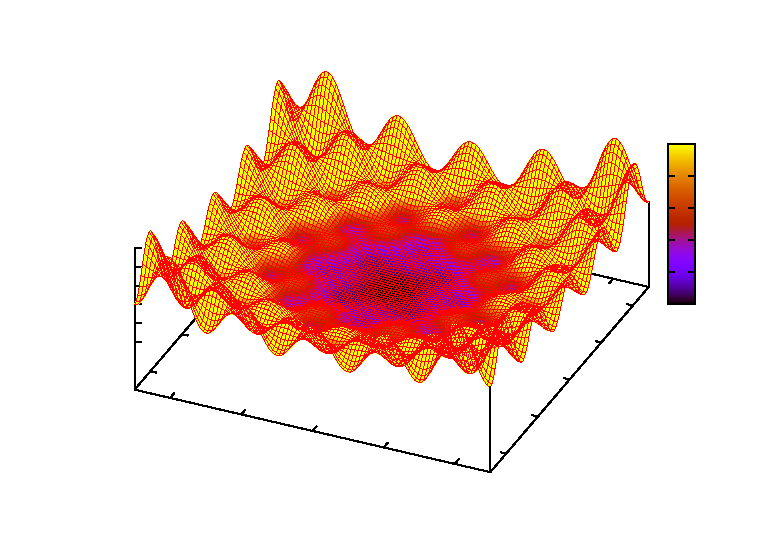
\includegraphics{qlws2014-gnuplottex-fig5}}%
    \gplfronttext
  \end{picture}%
\endgroup

\caption{test function for global optimization $\frac{\{\sin(\pi(x+\frac{1}{2}))\cos(\pi(y+1))+2\}(x^2+y^2)}{50}$}
\end{figure}
\end{minipage}}
}

\begin{frame}[fragile]
\frametitle{Comparison of optimizers}

\begin{table}
\begin{tabular}{l|c|c|r}
Optimizer & found minimum & target fct& \#evaluations \\
\hline
\verb Simplex & (2.965, 2.965) & 0.356 & 128 \\
\verb SimulatedAnnealing & (0.0, 0.0) & 0.0 & 10962 \\
\verb DifferentialEvolution & (0.0, 0.0) & 0.0 & 500700
\end{tabular}
\end{table}

\begin{enumerate}
\item Nelder-Mead lambda $= 0.2$
\item Start Temperature for simulated annealing is $T=1.0$ and decreased by a factor of $0.9$ each $5$ optimization steps
\item Configuration for DE is the default one
\end{enumerate}
 
\end{frame}

\section{Runge Kutta ODE Solver}

\frame{\frametitle{Runge Kutta ODE Solver}
An ODE solver using a forth order Runge Kutta scheme with adaptive step size control (as described in Numerical Recipes in C, Chapter 17.2). It integrates

\begin{equation}
\frac{d}{dx}f = F(x,f(x))
\end{equation}

over an interval $[a,b]$ for $f:[a,b]\rightarrow \mathbb{K}^n$ with $\mathbb{K}$ denoting the real or complex numbers with initial condition $f(a)=f_a$.
}

\begin{frame}[fragile]
\frametitle{Solving the modified Bessel equation}
As an example we solve the modified Bessel equation

\begin{equation}\label{modBessel}
x^2y''+xy'-(x^2+\alpha²)y = 0
\end{equation}

for $\alpha=1$ with $y(0)=0$ and $y'(0)=0.5$ over $[0,10]$ and compare it to the expected result $I_\alpha(10)$ (\verb+modifiedBesselFunction_i+).
\end{frame}

\begin{frame}[fragile]
\frametitle{Reduction to first derivatives}
Equation \ref{modBessel} is equivalent to the system
\begin{eqnarray}
y' = z \\
x^2z'+xz-(x^2+\alpha²)y = 0
\end{eqnarray}

with $y(0)=0$ and $z(0)=y'(0)=0.5$.
\end{frame}

\begin{frame}[fragile]
\frametitle{Code example for ODE solving}
The ODE $F$ can be defined as follows:
\vspace{2mm}
\begin{minted}[bgcolor=mintedBg,fontsize=\footnotesize]{c++}
Disposable<std::vector<Real>> rhs(const double x, 
                                   const std::vector<Real> &f) {
    std::vector<Real> result(2);
    result[0] = f[1];
    if (close(x, 0.0))
        result[1] = (2.0 + alpha * alpha) * f[0] / 2.0;
    else
        result[1] = ((x * x + alpha * alpha) *
                          f[0] - x * f[1]) / (x * x);
    return result;
}
\end{minted}

\end{frame}

\begin{frame}[fragile]
\frametitle{Code example for ODE solving}
To compute $I_1(10)$ we can then write
\vspace{2mm}
\begin{minted}[bgcolor=mintedBg,fontsize=\footnotesize]{c++}
AdaptiveRungeKutta<Real> rk( 1e-16 );
std::vector<Real> y;
y += 0.0, 0.5;
Real i1 = rk( rhs, y , 0.0, 10.0 )[0];
\end{minted}
\\
\vspace{2mm}
with an ultra-tight tolerance here, just to see what is possible.
\end{frame}

% %just to generate figure that is included below
% \begin{frame}[fragile]
% \begin{figure}
% 	 \begin{gnuplot}
%        set terminal epslatex color
%        set xrange [0.0:10.0]
%        set yrange [*:*]
%        set xlabel "x"
%        set ylabel "error"
%        unset key
%        set logscale y
%        set format y "%1.0e"
%        plot 'out7.txt' u 1:(abs($2-$3)) w l
% 	 \end{gnuplot}
% \end{figure}
% \end{frame}


\frame{\frametitle{ODE solution vs. semi-analytical solution}
\resizebox{\textwidth}{!}{
\begin{minipage}{1.5\textwidth}
\begin{figure}
% GNUPLOT: LaTeX picture with Postscript
\begingroup
  \makeatletter
  \providecommand\color[2][]{%
    \GenericError{(gnuplot) \space\space\space\@spaces}{%
      Package color not loaded in conjunction with
      terminal option `colourtext'%
    }{See the gnuplot documentation for explanation.%
    }{Either use 'blacktext' in gnuplot or load the package
      color.sty in LaTeX.}%
    \renewcommand\color[2][]{}%
  }%
  \providecommand\includegraphics[2][]{%
    \GenericError{(gnuplot) \space\space\space\@spaces}{%
      Package graphicx or graphics not loaded%
    }{See the gnuplot documentation for explanation.%
    }{The gnuplot epslatex terminal needs graphicx.sty or graphics.sty.}%
    \renewcommand\includegraphics[2][]{}%
  }%
  \providecommand\rotatebox[2]{#2}%
  \@ifundefined{ifGPcolor}{%
    \newif\ifGPcolor
    \GPcolortrue
  }{}%
  \@ifundefined{ifGPblacktext}{%
    \newif\ifGPblacktext
    \GPblacktexttrue
  }{}%
  % define a \g@addto@macro without @ in the name:
  \let\gplgaddtomacro\g@addto@macro
  % define empty templates for all commands taking text:
  \gdef\gplbacktext{}%
  \gdef\gplfronttext{}%
  \makeatother
  \ifGPblacktext
    % no textcolor at all
    \def\colorrgb#1{}%
    \def\colorgray#1{}%
  \else
    % gray or color?
    \ifGPcolor
      \def\colorrgb#1{\color[rgb]{#1}}%
      \def\colorgray#1{\color[gray]{#1}}%
      \expandafter\def\csname LTw\endcsname{\color{white}}%
      \expandafter\def\csname LTb\endcsname{\color{black}}%
      \expandafter\def\csname LTa\endcsname{\color{black}}%
      \expandafter\def\csname LT0\endcsname{\color[rgb]{1,0,0}}%
      \expandafter\def\csname LT1\endcsname{\color[rgb]{0,1,0}}%
      \expandafter\def\csname LT2\endcsname{\color[rgb]{0,0,1}}%
      \expandafter\def\csname LT3\endcsname{\color[rgb]{1,0,1}}%
      \expandafter\def\csname LT4\endcsname{\color[rgb]{0,1,1}}%
      \expandafter\def\csname LT5\endcsname{\color[rgb]{1,1,0}}%
      \expandafter\def\csname LT6\endcsname{\color[rgb]{0,0,0}}%
      \expandafter\def\csname LT7\endcsname{\color[rgb]{1,0.3,0}}%
      \expandafter\def\csname LT8\endcsname{\color[rgb]{0.5,0.5,0.5}}%
    \else
      % gray
      \def\colorrgb#1{\color{black}}%
      \def\colorgray#1{\color[gray]{#1}}%
      \expandafter\def\csname LTw\endcsname{\color{white}}%
      \expandafter\def\csname LTb\endcsname{\color{black}}%
      \expandafter\def\csname LTa\endcsname{\color{black}}%
      \expandafter\def\csname LT0\endcsname{\color{black}}%
      \expandafter\def\csname LT1\endcsname{\color{black}}%
      \expandafter\def\csname LT2\endcsname{\color{black}}%
      \expandafter\def\csname LT3\endcsname{\color{black}}%
      \expandafter\def\csname LT4\endcsname{\color{black}}%
      \expandafter\def\csname LT5\endcsname{\color{black}}%
      \expandafter\def\csname LT6\endcsname{\color{black}}%
      \expandafter\def\csname LT7\endcsname{\color{black}}%
      \expandafter\def\csname LT8\endcsname{\color{black}}%
    \fi
  \fi
  \setlength{\unitlength}{0.0500bp}%
  \begin{picture}(7200.00,5040.00)%
    \gplgaddtomacro\gplbacktext{%
      \csname LTb\endcsname%
      \put(1078,704){\makebox(0,0)[r]{\strut{}1e-17}}%
      \put(1078,1286){\makebox(0,0)[r]{\strut{}1e-16}}%
      \put(1078,1867){\makebox(0,0)[r]{\strut{}1e-15}}%
      \put(1078,2449){\makebox(0,0)[r]{\strut{}1e-14}}%
      \put(1078,3030){\makebox(0,0)[r]{\strut{}1e-13}}%
      \put(1078,3612){\makebox(0,0)[r]{\strut{}1e-12}}%
      \put(1078,4193){\makebox(0,0)[r]{\strut{}1e-11}}%
      \put(1078,4775){\makebox(0,0)[r]{\strut{}1e-10}}%
      \put(1210,484){\makebox(0,0){\strut{} 0}}%
      \put(2329,484){\makebox(0,0){\strut{} 2}}%
      \put(3447,484){\makebox(0,0){\strut{} 4}}%
      \put(4566,484){\makebox(0,0){\strut{} 6}}%
      \put(5684,484){\makebox(0,0){\strut{} 8}}%
      \put(6803,484){\makebox(0,0){\strut{} 10}}%
      \put(176,2739){\rotatebox{-270}{\makebox(0,0){\strut{}error}}}%
      \put(4006,154){\makebox(0,0){\strut{}x}}%
    }%
    \gplgaddtomacro\gplfronttext{%
    }%
    \gplbacktext
    \put(0,0){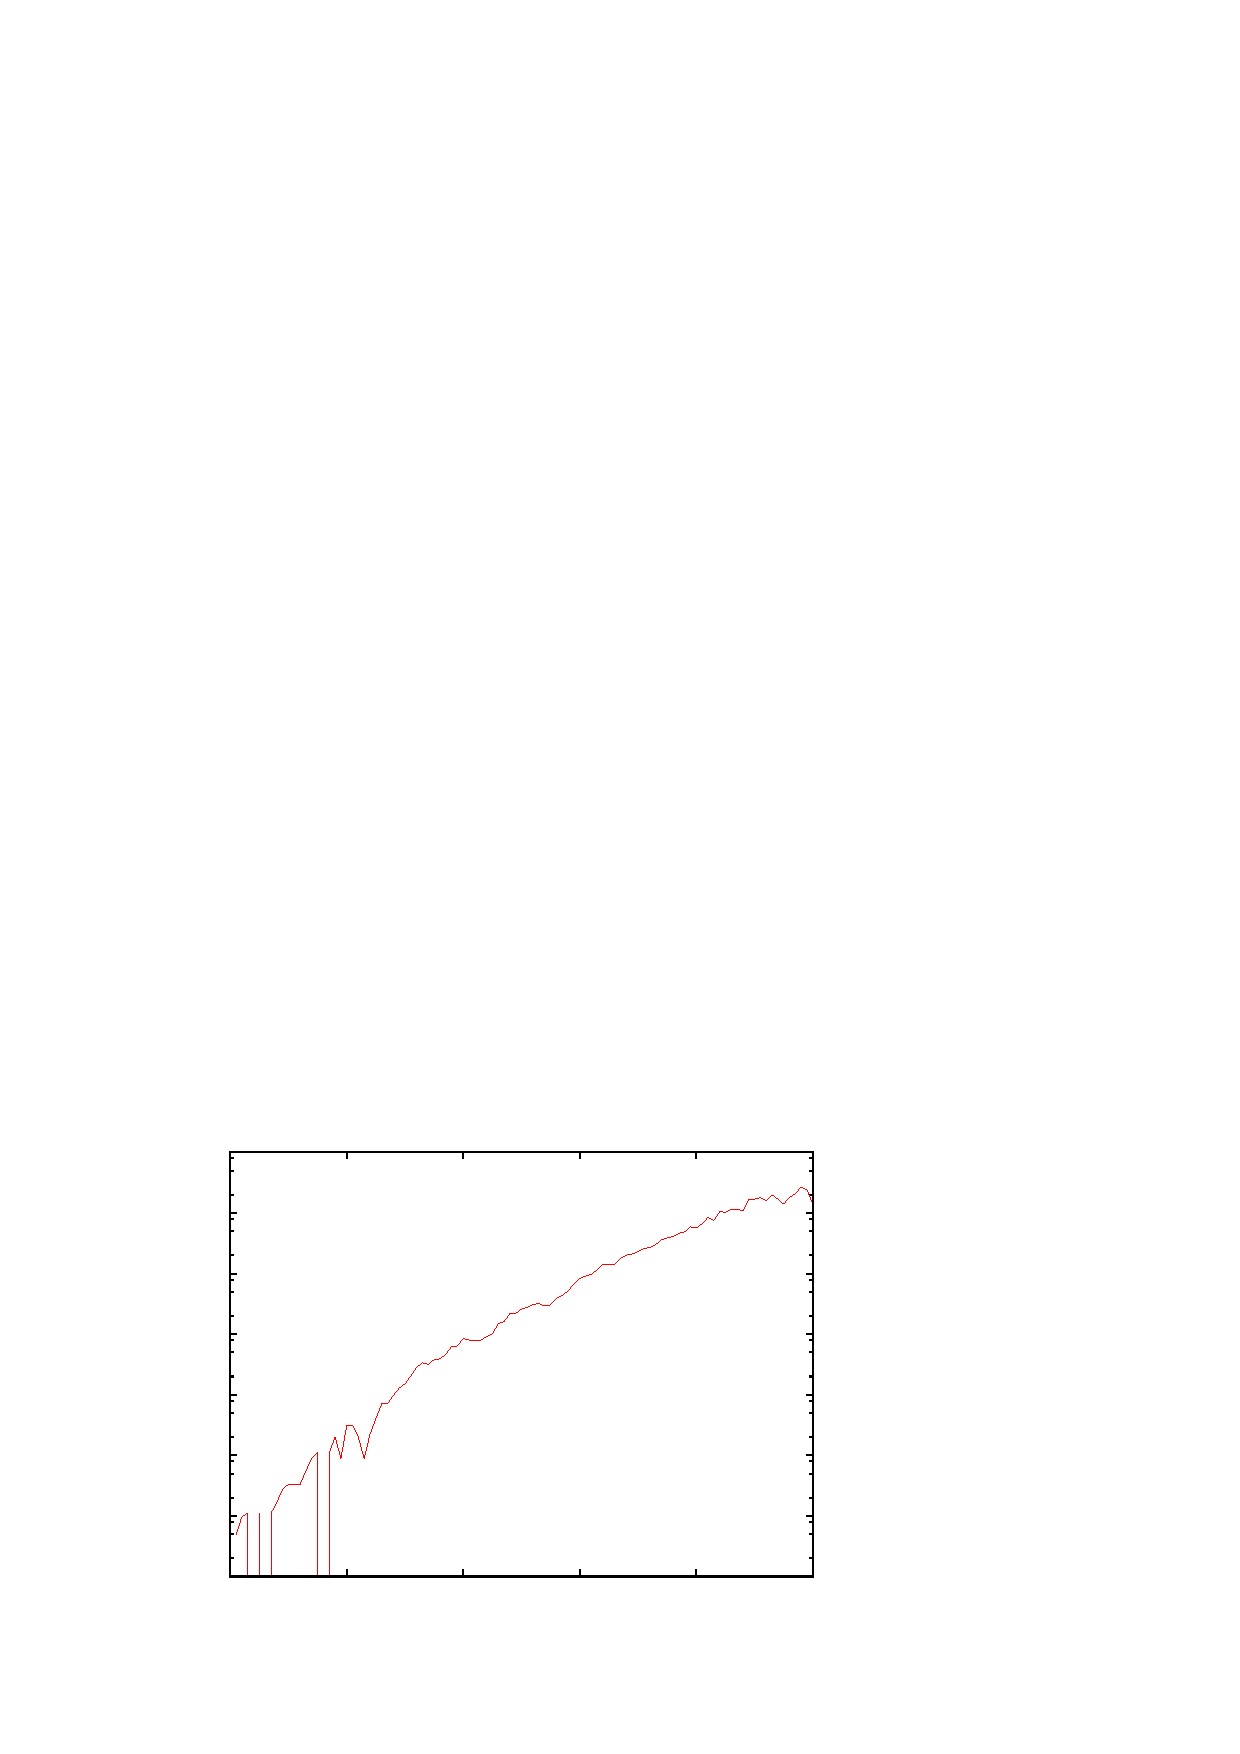
\includegraphics{qlws2014-gnuplottex-fig6}}%
    \gplfronttext
  \end{picture}%
\endgroup

\caption{Runge Kutta adaptive step size solution with $\epsilon=10^{-16}$ vs. modifiedBessel\_i}
\end{figure}
\end{minipage}}
}



\section{Dynamic Creator of Mersenne Twister}

\begin{frame}[fragile]
\frametitle{Dynamic Creator of Mersenne Twister}

Makoto Matsumoto and Takuji Nishimura, ``Dynamic Creation of Pseudorandom Number Generators'' and their implementation as a C library (http://www.math.sci.hiroshima-u.ac.jp/\~{}m-mat/MT/DC/dc.html) addresses two needs

\begin{enumerate}
\item create Mersenne Twister instances with smaller state space than the classic instance (624 words of 32 bit) and smaller period than $2^{19937}-1$, or bigger ones if you really want ...
\item create ``independent'' Mersenne Twister intances for different id's for use in parralel monte carlo
\end{enumerate}

The QuantLib wrapper support both dynamic creation of instances (\verb+MersenneTwisterDynamicRng+) as well as the usage of precomputed instances (\verb+MersenneTwisterCustomRng<Description>+).
\end{frame}

\begin{frame}[fragile]
\frametitle{Instantiation of dynamic MT's}
Dynamically create an instance with 32 bit word size, $p=521$, creator seed $123$, id $0$ and seed $42$:
\vspace{2mm}
\begin{minted}[bgcolor=mintedBg]{c++}
MersenneTwisterDynamicRng mt(32,521, 123, 0, 42);
\end{minted}

Use a precomputed instance with seed $42$ ($p$ is $19937$ here, id is $0$)
\vspace{2mm}
\begin{minted}[bgcolor=mintedBg]{c++}
MersenneTwisterCustomRng<Mtdesc19937_0> mt(42);
\end{minted}

The second alternative is much faster in random number generation. Also it takes a long time to dynamically create MT instances for bigger $p$.
\end{frame}


\begin{frame}[fragile]
\frametitle{Example: Parallel RNG streams}
This code computes $\pi$ using parallel mc with $8$ threads
\vspace{2mm}
\begin{minted}[bgcolor=mintedBg,fontsize=\tiny]{c++}
#define BOOST_PP_LOCAL_LIMITS (0, 7)
#define BOOST_PP_LOCAL_MACRO(n) MersenneTwisterCustomRng<Mtdesc19937_##n> mt##n(42);
#include BOOST_PP_LOCAL_ITERATE()
    omp_set_num_threads(std::min(8, omp_get_max_threads()));
    Real sum = 0.0;
    Size N = 1E8;
#pragma omp parallel for reduction(+ : sum) schedule(static)
    for (Size i = 0; i < N; ++i) {
        Size thread = omp_get_thread_num();
        Real u=0.0,v=0.0;
#define BOOST_PP_LOCAL_LIMITS (0, 7)
#define BOOST_PP_LOCAL_MACRO(n) if(thread==n) { u=mt##n.nextReal(); v=mt##n.nextReal(); }
#include BOOST_PP_LOCAL_ITERATE()
        if(u*u+v*v <= 1.0) sum+=1;
    }
    std::cout << std::setprecision(8) << 4.0 * sum / N << std::endl;
\end{minted}

Actually this does not run faster multithreaded due to compiler optimizations (vectorization) of the loop, nevertheless illustrates how to use it.
\end{frame}

\frame{\frametitle{What does ``independent'' mean ? (1/2)}
The MT sequence can be seen as a recurrence

\begin{eqnarray}
s_{n} = As_{n-1} \\
x_{n} = Bs_n 
\end{eqnarray}

with a state transition matrix $A$ and an output transformation matrix $B$. $s_n$ satisfies the following equation in $\mathbb{F}_2^k$, $k$ being the bit size of the state space

\begin{equation}
\chi(A) s_{n-k} = 0
\end{equation}

with the characteristic polynomial $\chi$ of $A$ (Cayley Hamilton Theorem).
}

\frame{\frametitle{What does ``independent'' mean ? (2/2)}
Two independent MT instances have by definition coprime characteristic polynomials $f$, $g$, thus there is an isomorphism of the residual polynomial rings (thanks to the chinese remainder theorem)

\begin{equation}
\mathbb{F}_2[T] / (fg) \cong \mathbb{F}_2[T] / (f) \times \mathbb{F}_2[T] / (g)
\end{equation}

which is formalizing what independdence of the recurrences of the two MT instances mean.

}



\section{Questions}

\begin{frame}[fragile]
\frametitle{Questions / Discussion}
\resizebox{\textwidth}{!}{
\begin{minipage}{0.75\textwidth}
\begin{figure}
	\centering
		\includegraphics{../../../Pictures/erlkoenige/french_70s_automodule05.jpg}
\end{figure}
\end{minipage}}
\\
\begin{center}
French Erlk\"onig
\end{center}
\end{frame}
\end{document}

